\section{Introduction}
Acoustic scattering is a large field which has one of its application in the analysis of scattering on submarines. The scattering problem is by no means limited to submarines, as the physical phenomena occurs all around in nature. For instance, acoustic scattering may be used to calculate the number of fish in a fish farming net~\cite{conti2006amo}. Moreover, the fluid to be analyzed is not limited to be water. For acoustic scattering problems, the Helmholtz equation represents the governing equation for the fluid medium. The same equation in vector form can govern electromagnetic waves (see~\cite{Manh2012iaa}).

The problem at hand is time dependent. But we shall assume harmonic time dependency, such that all time dependent functions $\breve{F}=\breve{F}(\vec{x},t)$ may be written as
\begin{equation}\label{Eq4:periodicityAssumption}
	\breve{F}(\vec{x}, t) = F(\vec{x})\euler^{-\imag\omega t}
\end{equation}
where $\omega$ is the angular frequency and $\imag = \sqrt{-1}$ the imaginary unit. This enables us to model the pressure $p$ in the fluid with the Helmholtz equation given by
\begin{equation}\label{Eq4:HelmholtzEquationIntro}
	\nabla^2 p + k^2 p = 0
\end{equation}
with the wave number $k=\frac{\omega}{c_{\mathrm{f}}}$ (where $c_{\mathrm{f}}$ is the wave speed in the fluid). Other important quantities include the frequency $f=\frac{\omega}{2\pi}$ and the wavelength $\lambda = \frac{2\pi}{k}$.

By assuming the normal derivative of the total pressure at the boundary to be given by a physical optics approximation, the Kirchoff approximation enables efficient computation of the scattered pressure from objects. This approximation is best suited for smooth convex objects as edges and multiple reflections are not well approximated using this approach~\cite{Fawcett2001moh}. The Kirchhoff approximation has also been used to model problems in the time domain~\cite{Fawcett2001moh, Pouliquen1999tem}. For a more detailed introduction to this method, we refer to~\cite{Medwin1997foa}.

The geometry of the scatterer may be quite complex but is typically exactly represented using Non-Uniform Rational B-Splines (NURBS). This fact is one of the motivations of using the isogeometric analysis (IGA) concept as it uses the same functions as basis function for analysis. The sphere depicted in \Cref{Fig4:SphericalShellCAD} is an example of a geometry which has an exact representation using NURBS.
\begin{figure}
	\centering
	\begin{subfigure}[t]{0.3\textwidth}
		\centering
		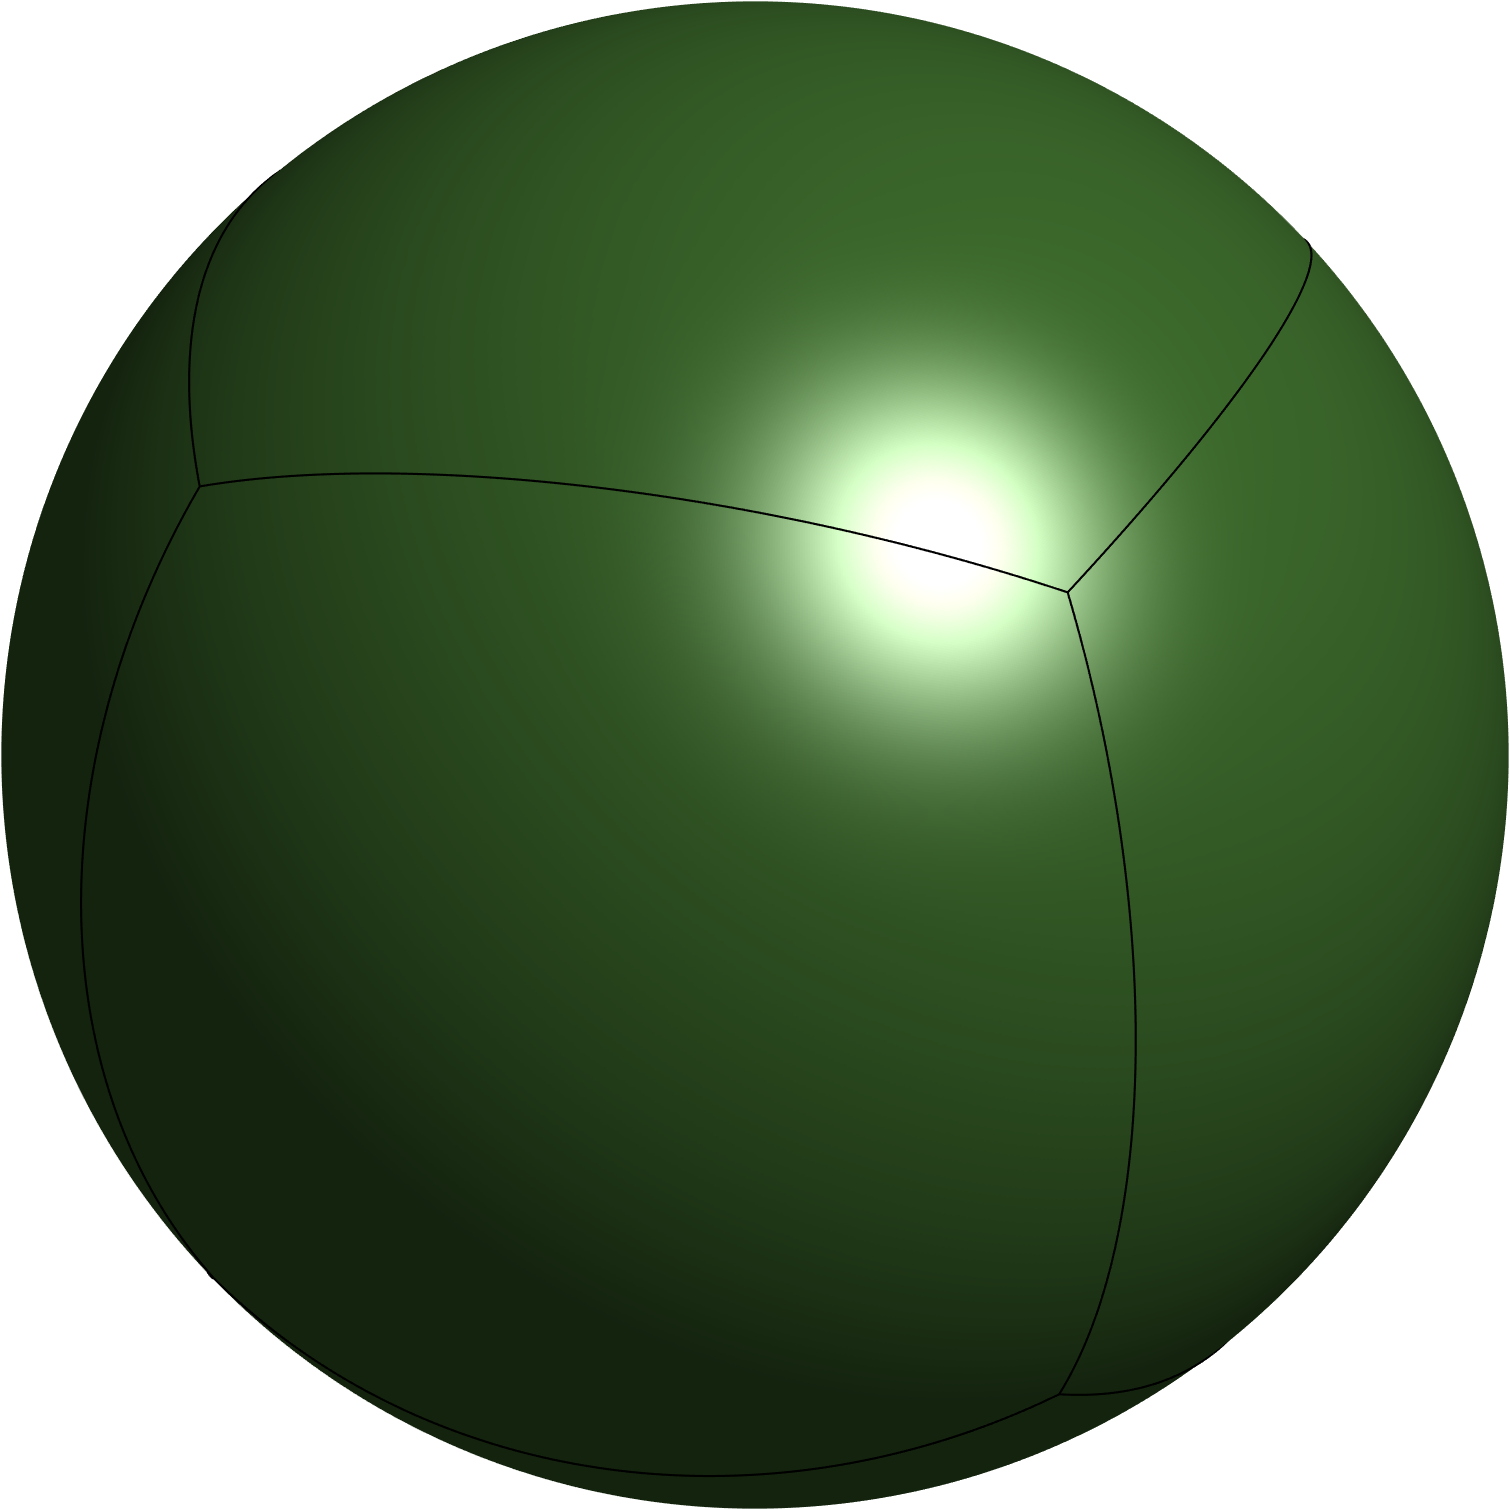
\includegraphics[width=0.9\textwidth]{S1patched}
		\caption{Exact CAD model.}
		\label{Fig4:SphericalShellCAD}
	\end{subfigure}
	~
	\begin{subfigure}[t]{0.3\textwidth}
		\centering
		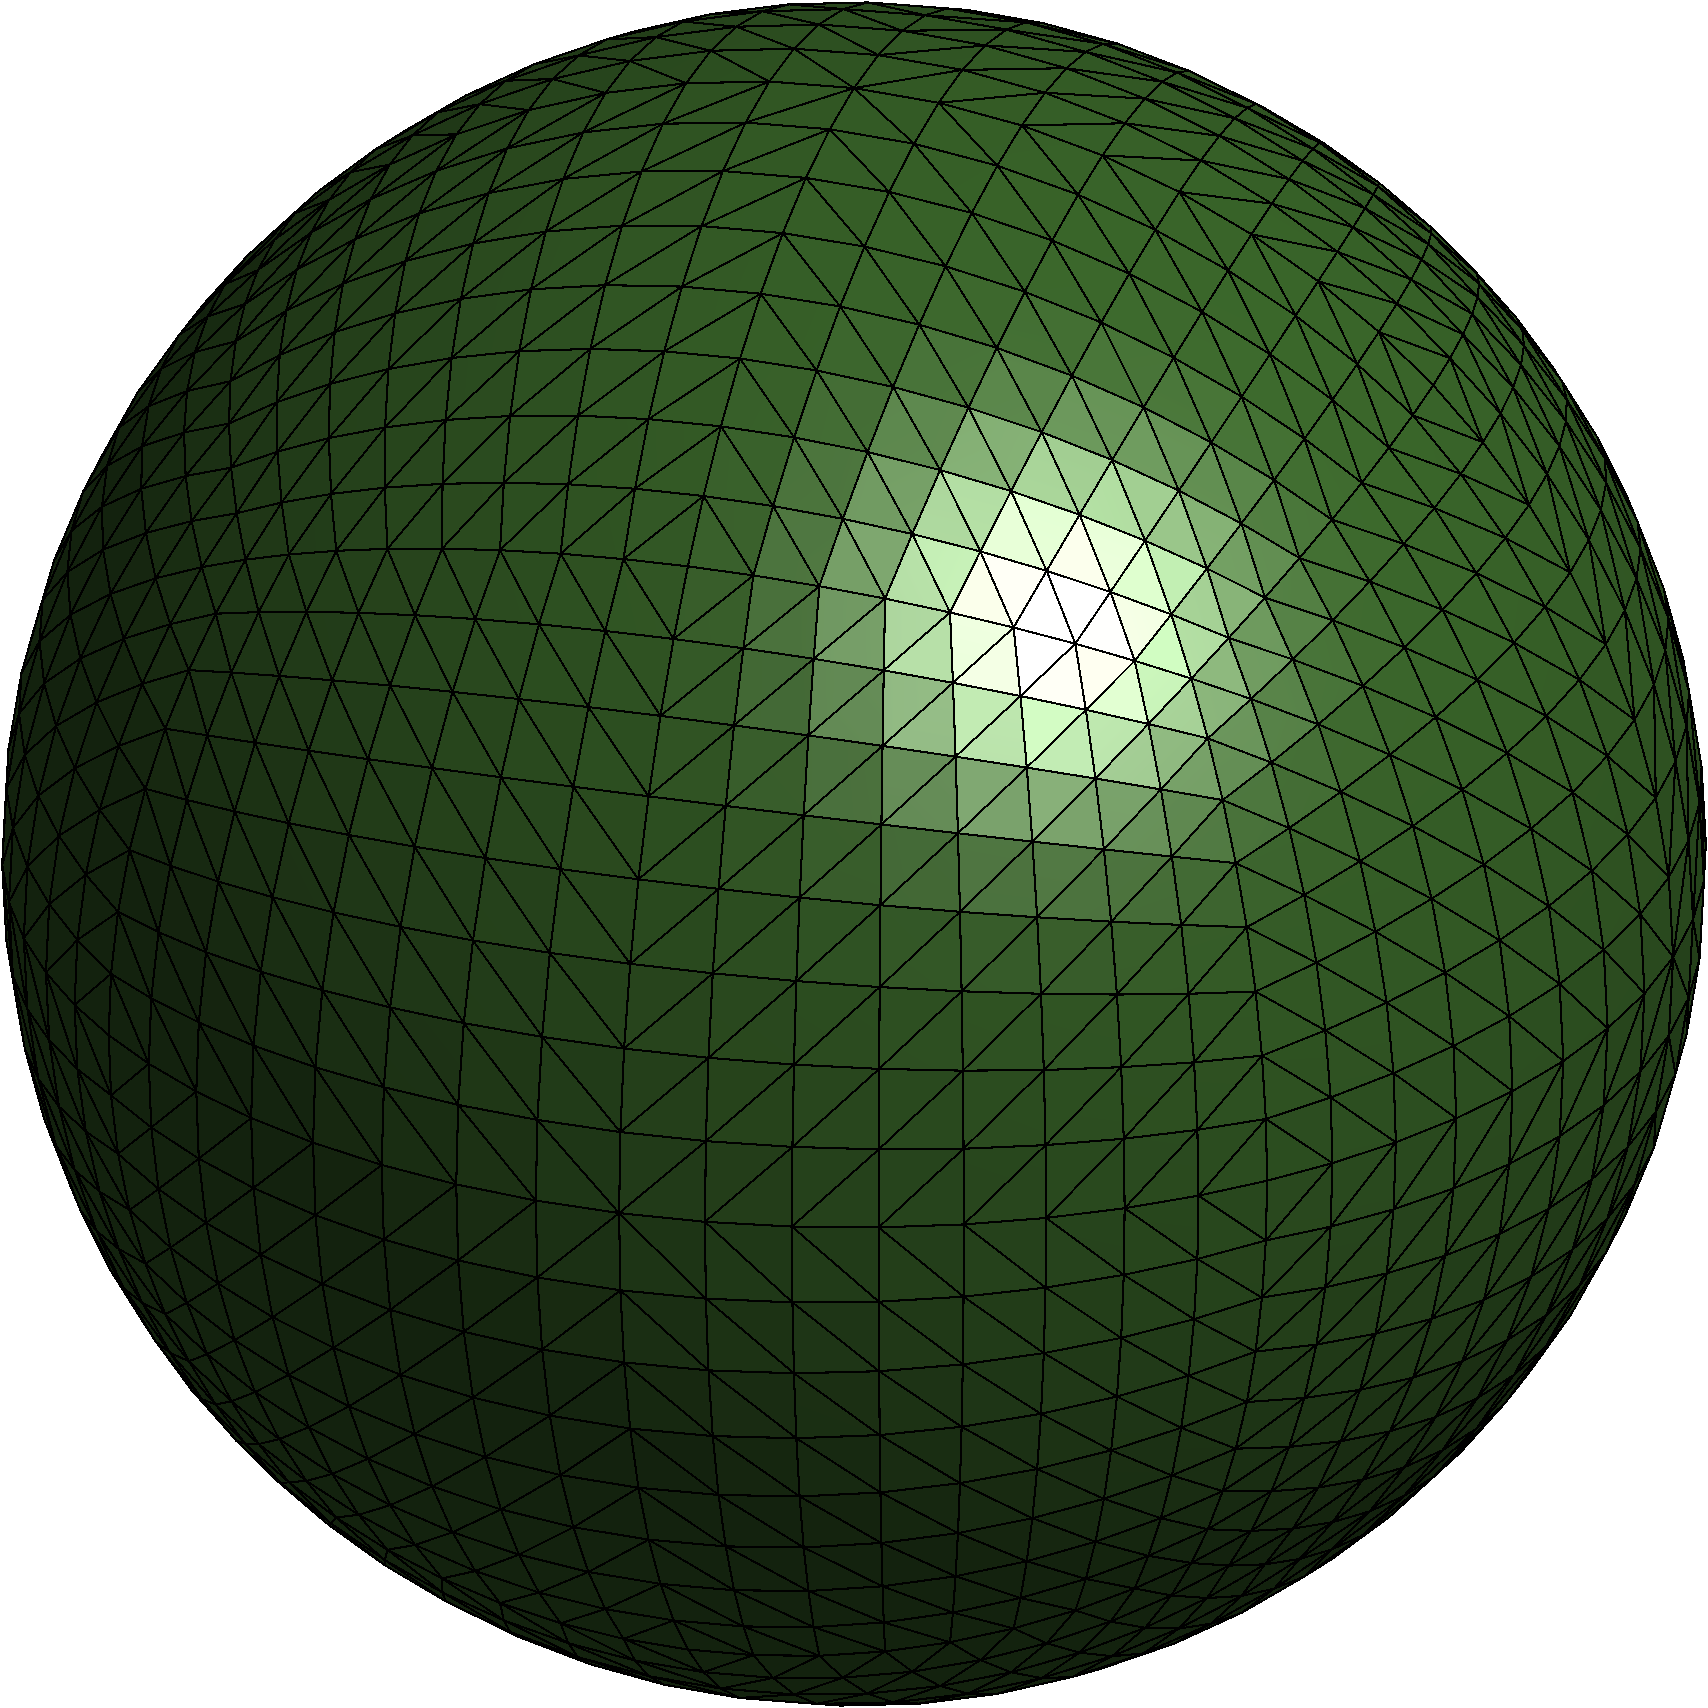
\includegraphics[width=0.9\textwidth]{trianglesParm2_3072}
		\caption{Triangulation with 3072 triangles.}
		\label{Fig4:SphericalShellTriangles1}
	\end{subfigure}
	~
	\begin{subfigure}[t]{0.3\textwidth}
		\centering
		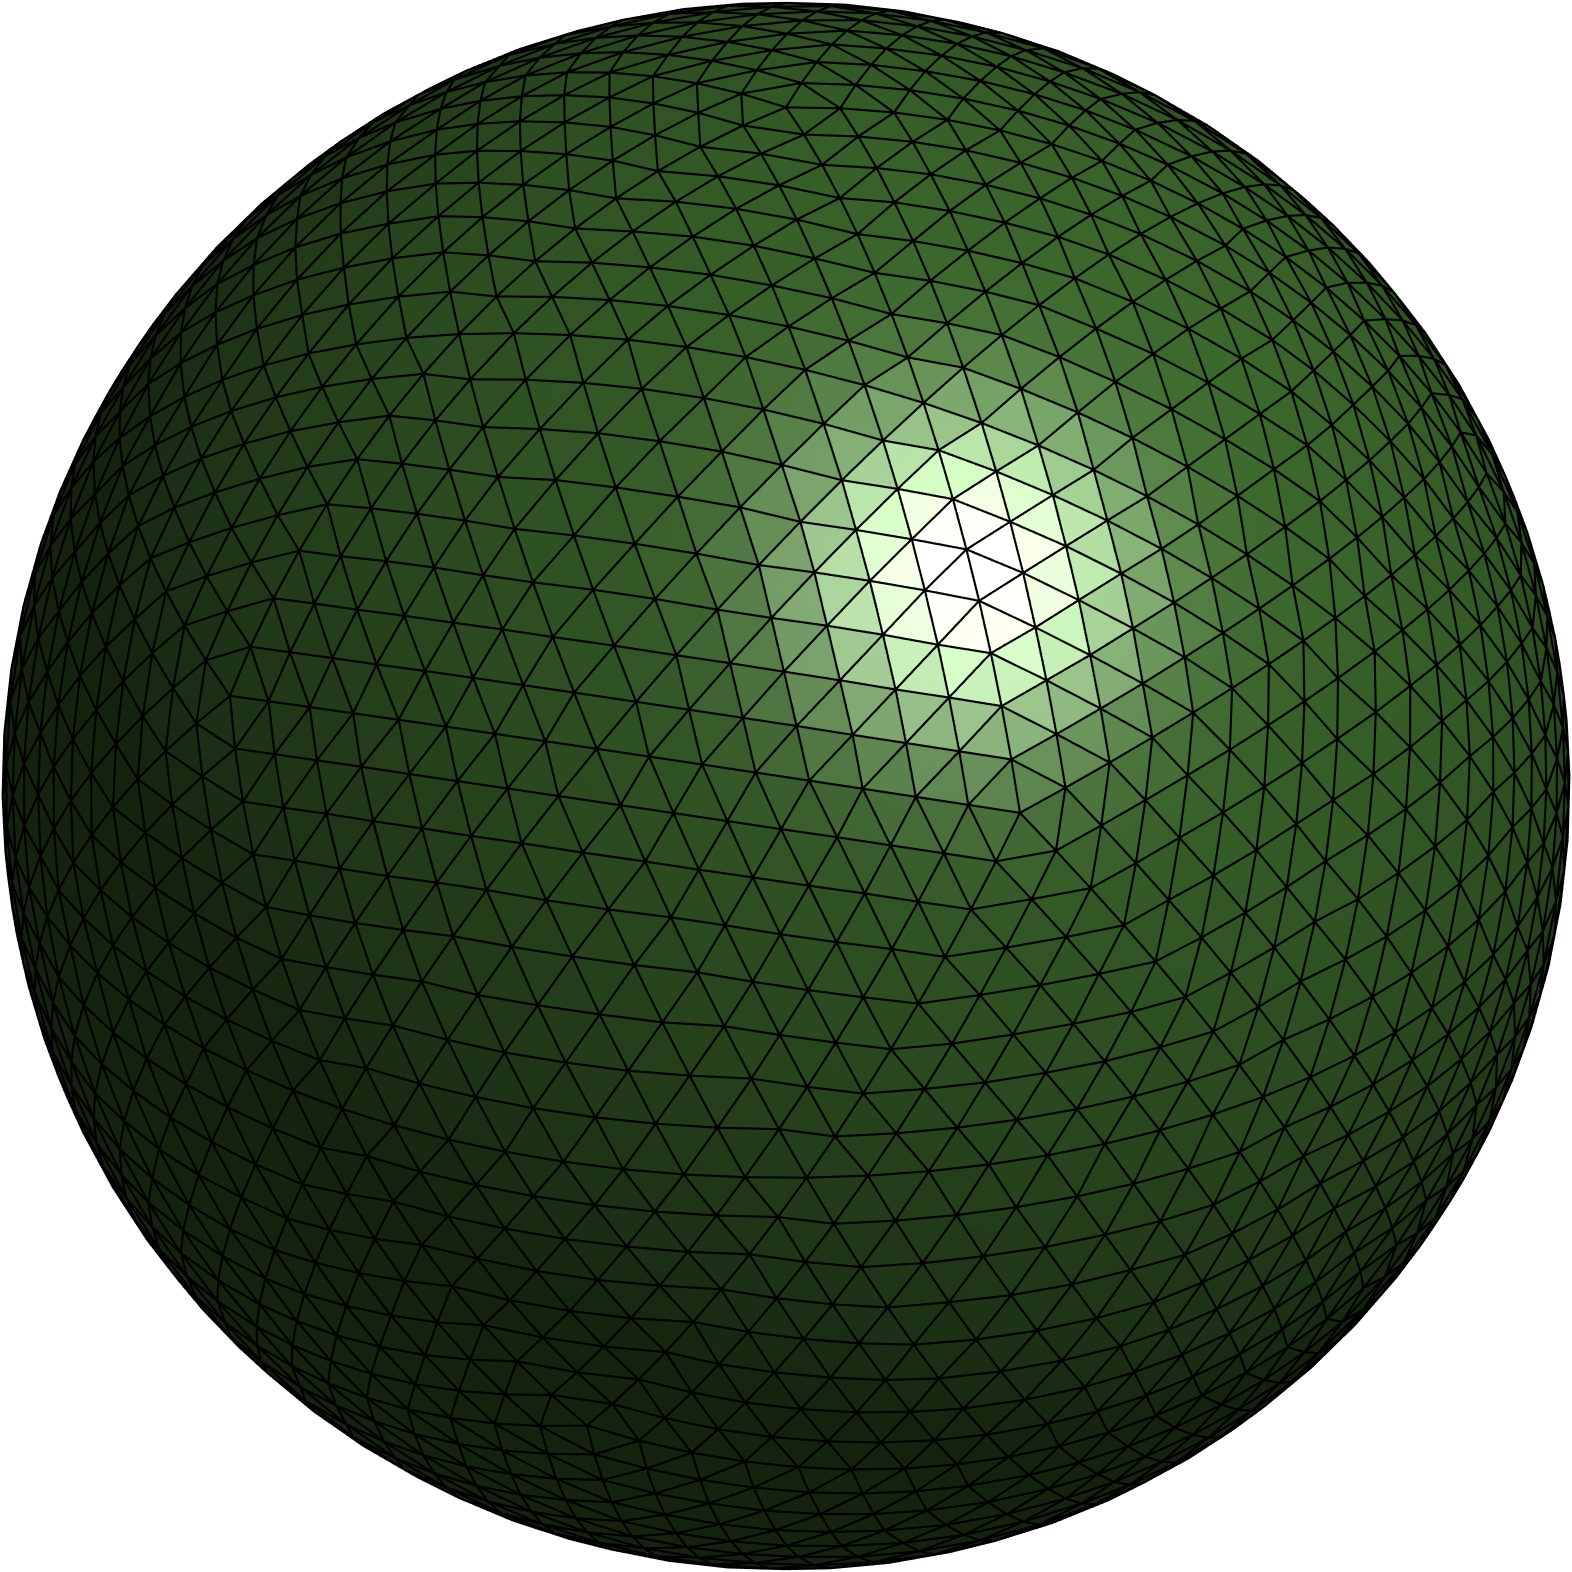
\includegraphics[width=0.9\textwidth]{triangles}
		\caption{Triangulation with 5120 triangles.}
		\label{Fig4:SphericalShellTriangles2}
	\end{subfigure}
	\caption{A CAD model often uses spline-based parametrization for modeling. Analysis are often made on an approximation of such a geometry. The surface of a sphere may be modeled by 6 patches using NURBS parametrizations.}
	\label{Fig4:SphericalShell}
\end{figure} 
A triangulation of such a geometry can easily be obtained by refining the CAD model, and then use the element corners as nodes for the triangulation as in \Cref{Fig4:SphericalShellTriangles1}. This may result in non-optimal triangulation as the triangles should be as close as possible to equilateral triangles of equal size (\Cref{Fig4:SphericalShellTriangles2}). 

The approach of triangularization approximation has been used quite extensively in the BeTSSi\footnote{Benchmark Target Strength Simulation \cite{Nolte2014bib}.} community \cite{Schneider2003asb,Fillinger2014aen,Oestberg2016tes,Gilroy2017tes} as the integration over triangles can be evaluated exactly. This approach is also taken in~\cite{Foote2002cka,Abawi2016ksf}. As reported in \cite{Gilroy2017tes} triangulating a submarine model for $\SI{30}{kHz}$ might result in a file size of several hundred GB. This is because the accuracy is frequency dependent when approximating the geometry. In \cite{Foote2002cka} the integration was done using classical Gauss quadrature where they suggest the maximal point separation to be $\lambda/6$. A similar approach was taken in~\cite{Pignier2015aka} where the maximal point separation was taken to be $\lambda/4$. This leads to computationally expensive calculations for high frequencies. An attempt to solve the problem of high memory consumption and low accuracy for high frequencies was made in~\cite{Lavia2018mhf} where a hybrid method was proposed using Gaussian quadrature on curvilinear facets. This approach seems to reduce the number of required facets by a significant amount (although still having frequency dependent accuracy). The main disadvantage is here arguably the requirement of tessellation of the CAD model into curvilinear facets. 

In this work we will take the approach of using the exact geometry and using the numerical steepest descent to perform highly oscillatory integration, which is an attempt to solve the two problems of memory and accuracy dependency of large frequencies in addition to avoiding the tessellation process altogether using the IGA framework. The advantages of using curvilinear facets are covered indirectly in this work as one can choose to use classical Gauss-Legendre quadrature (on a refined IGA mesh) to evaluate the oscillatory integrals instead of the numerical steepest descent.

The integrals investigated in this work are related to the boundary integrals used in the boundary element method (BEM). Especially the approach by Peake et al.~\cite{Peake2015eib} where the NURBS basis functions are enriched with oscillatory plane waves. Peake evaluated the resulting integral using high order Gauss Legendre quadrature, which will be the bottleneck for high frequencies. This work sets a foundation for solving this problem using NSD.

The problem of highly oscillatory integration has long been an active research area. Especially integrals of the form
\begin{equation}\label{Eq4:oscillatoryIntegral}
	I[f,\Omega]=\int_{\Omega} f(\vec{x})\euler^{\imag \omega g(\vec{x})}\idiff \Omega
\end{equation}
are of major interest. Here $\Omega\subset\R^d$ is usually a bounded open domain with piece-wise smooth boundary, while the \textit{amplitude function} $f$ and the \textit{oscillator} $g$ are smooth. The integral in \Cref{Eq4:oscillatoryIntegral}, is highly oscillatory for large values of $\omega\in\R$. Integration of such highly oscillatory integrals using classical Gaussian quadrature becomes prohibitively computationally expensive for large $\omega$, and one should resort to other methods. Alternative methods such as asymptotic methods and Filon-type methods~\cite{Dominguez2011sae,Iserles2004oqm,Iserles2005eqo}, Levin-type methods~\cite{Levin1996fio,Olver2006mfn}, numerical steepest descent~\cite{Huybrechs2006ote,Deano2018cho}, complex Gaussian quadrature~\cite{Asheim2013cgq,Deano2015tkp} have attained great interest during the last decade and we refer to the book by Dea{\~{n}}o et al.~\cite{Deano2018cho} for more details. 

In~\Cref{Sec4:Kirchhoffs} we start by briefly presenting the Kirchhoff approximation, and continue by presenting the numerical steepest descent in \Cref{Sec4:NumericalSteepestDecent}. Numerical examples are presented in \Cref{Sec4:resultsAndDiscussion} followed by the conclusions in \Cref{Sec4:conclusions}.